\newpage
\section{Chapter 2}

\begin{multicols}{2}
\setlength{\columnsep}{1.5cm}
\setlength{\columnseprule}{0.2pt}

\subsection{DFA: Deterministic Finite Automata}

\begin{definition}{}
  A \textbf{deterministic finite automaton} is a quintuple $M = (K, \Sigma, \delta, s, F)$ where
  \begin{itemize}
    \item $K$ is a finite set of \textbf{states}
    \item $\Sigma$ is an alphabet,
    \item $s \in K$ is the \textbf{initial state}
    \item $F \subseteq K$ is the set of \textbf{final states}
    \item $\delta$, the \textbf{transition function}, is a function from $K \times \Sigma$ to $K$. 
  \end{itemize}
\end{definition}

The \textbf{configuration} of the machine is the \textit{current state and the unread part of the input string}, i.e., a configuration is an element of $K \times \Sigma^*$.

Let $(q, w)$ and $(q',w')$ be two configurations of $M$. Then $(q, w) \vdash_M (q', w')$ if and only if $w = aw'$ for some $a \in \Sigma$ and $q' = \delta(q, a)$. For example, $(q, aabb) \vdash_M (q', abb)$ where $q' = \delta(q, a)$.

$(q, w) \vdash_M (q', w')$ reads $(q, w)$ \textbf{yields} $(q', w')$ in \textbf{one step}. $\vdash^*_M$ is the \textbf{reflexive transitive closure} of $\vdash_M$ (It can be though like the multiple steps). A string $w \in \Sigma^*$ is \textbf{accepted} by $M$ if and only if $(s, w) \vdash^*_M (f, e)$ for some $f \in F$. The \textbf{language} of $M$, $L(M)$, is the set of strings \textit{accepted} by $M$.

\vfill\null
\columnbreak


\subsection{NFA: Nondeterministic Finite Automata}

\begin{definition}{}
  A \textbf{nondeterministic finite automaton} is a quintuple $M = (K, \Sigma, \Delta, s, F)$, where
  \begin{itemize}
    \item $K$ is a finite set of \textbf{states}
    \item $\Sigma$ is an alphabet
    \item $s \in K$ is the \textbf{initial state}
    \item $F \subseteq K$ is the set of \textbf{final states}, and
    \item $\Delta$, the \textbf{transition relation}, is a subset of $K \times (\Sigma \cup \{e\}) \times K$ 
\end{itemize}
\end{definition}

$(q, a, p) \in \Delta$ is called a \textbf{transition} of $M$. $(q, e, p)$ indicates that the machine can pass to state $p$ from state $q$ without reading an input symbol.

The \textbf{configuration} of the machine is the current state and the unread part of the input string, i.e., a configuration is an element of $K \times \Sigma^*$.

Let $(q, w)$ and $(q', w')$ be two configurations of $M$. Then $(q, w) \vdash_M (q', w')$ if and only if $w = aw'$ for some $a \in \Sigma \cup \{e\}$ and $(q, a, q') \in \Delta$.

$(q, w) \vdash_M (q', w')$ reads $(q, w)$ \textbf{yields} $(q', w')$ \textbf{in one step}. $\vdash^*_M$ is the \textbf{reflexive transitive closure} of $\vdash_M$. $(q, w) \vdash^*_M (q', w')$ reads $(q, w)$ yields $(q', w')$. A string $w \in \Sigma^*$ is \textbf{accepted} by $M$ if and only if there is a state $f \in F$ such that $(s, w) \vdash^*_M (f, e)$. The \textbf{language} of $M$, $L(M)$, is the set of strings accepted by $M$.

\textit{A deterministic finite state automaton is just a special type of nondeterministic finite state automaton}. We obtain a DFA when $\Delta$ defines a function from $K \times \Sigma$ to $K$. In other words, an NFA $M = (K, \Sigma, \Delta, s, F)$ is deterministic if there are no transitions of the form $(q, e, p)$ and for each $q \in K$ and $a \in \Sigma$, there exists \textit{exactly one} $p \in K$ such that $(q, a, p) \in \Delta$.

A nondeterministic finite automaton can always be converted to an \textit{equivalent} deterministic finite state automaton.

\begin{theorem}{}
  For each nondeterministic finite automaton, there exists an equivalent deterministic finite automaton.
\end{theorem}

Proof of the theorem is constructive. In proof, one can use subset construction algorithm to construct a DFA from anNFA and then show they are equivalent.

Two automaton (DFA or NFA, one can be DFA and the other can be NFA) $M_1$ and $M_2$ are said to be \textbf{equivalent} when $L(M_1) = L(M_2)$.

\end{multicols}

\newpage
\subsubsection{Subset Construction}

In here, the following is main and formal definition.

\begin{formula}{}
Given an NFA $M = (K, \Sigma, \Delta, s, F)$, the algorithm constructs an equivalent DFA $M' = (K', \Sigma, \delta, s', F')$ as follows. For each state $q \in K$, the set of states that can be reached without reading an input symbol is defined as
  \begin{align*}
    E(q) = \left\{ p \in K\ |\ (q, e) \vdash^*_M (p, e) \right\}
  \end{align*}
  Essentially, $E(q)$ is the reflexive transitive closure of the set $\left\{ q \right\}$ under the relation $\left\{(p, r)\ |\ (p, e, r) \in \Delta \right\}$. The DFA is defined as:
  \begin{align*}
    K' &= 2^K\\
    s' &= E(s)\\
    F' &= \left\{ Q \subseteq K\ |\ Q \cap F \neq \emptyset \right\}\\
    \delta'(Q, a) &= \left\{ E(p) : p \in K, (q, a, p) \in \Delta \textnormal{ for some } q \in Q \right\} \textnormal{ for each $Q \in K'$ and $a \in \Sigma$}\\
    &= \bigcup \left\{ E(p) : p \in K, (q, a, p) \in \Delta \textnormal{ for some } q \in Q \right\}
  \end{align*}
\end{formula}

\begin{multicols}{2}
\setlength{\columnsep}{1.5cm}
\setlength{\columnseprule}{0.2pt}

\begin{equation*}
  E(q) = \left\{ q \right\} \cup \left\{ p \in K\ |\ (q, e) \vdash^*_M (p, e) \right\}
\end{equation*}

If there is question about transforming an NFA to a DFA, the following steps can be used in question solving:
\begin{formula}{}
  \begin{enumerate}
    \item The NFA $M = (K, \Sigma, \Delta, s, F)$ is given and we want to construct DFA. In other words we want to acquire:
    \begin{equation*}
        M' = (K', \Sigma, \delta', s', F')
    \end{equation*}
    
    \item Start from the initial state of NFA, $s' = E(s)$. For each $q_j \in E(s)$ find the transition for each $k \in \Sigma$ ($q_j, k, q_l$).

    For example, if $E(s) = \{ q_{0}, q_{1} \}$. Look the transition from $q_0$ and $q_1$. If $\Sigma = \{ a, b \}$, then look for $a$ and $b$.
    
    
    \item Then calculate the union of $E(q_i)$ of the reachable states from the state we consider.
    
    For example, if transitions for $a$ are $(q_{0}, a, q_{1}), (q_{1}, a, q_{2})$, then write 
    \begin{quote}
      $(q_{0}, a, q_{1}), (q_{1}, a, q_{2})$ are all the transitions $(q, a, p)$ for some $q \in E(s)$
    \end{quote}
    and calculate the $\delta'(s', a) = E(q_{1}) \cup E(q_{2})$. If it is new state, write this new state on DFA, if not connect it the old one.
    
    \item Follow this steps for each $k \in \Sigma$ and newly introduced steps.
  \end{enumerate}
\end{formula}

\vfill\null
\columnbreak

Look at the example below, it is taken from 2.2.4 in the textbook.

\begin{example}{: NFA to DFA}
  For this example:
  \begin{itemize}
    \item $E(q_0) = \left\{ q_0, q_1, q_2, q_3  \right\}$
    \item $E(q_1) = \left\{ {q_1, q_2, q_3} \right\}$
    \item $E(q_2) = \left\{ q_2 \right\}$
    \item $E(q_3) = \left\{ q_3 \right\}$
    \item $E(q_4) = \left\{ q_3, q_4 \right\}$
  \end{itemize}
  
  \hfill\break

  $s' = E(q_0) = \left\{ q_0, q_1, q_2, q_3  \right\}$,
  \begin{equation*}
    (q_1, a, q_0),\ (q_1, a, q_4), \textnormal{ and } (q_3, a, q_4)
  \end{equation*}
  are all the transitions $(q, a, p)$ for some $q \in s'$. It follows that (Instead of $s'$ any state symbol can be used such as $q_{100}$)
  \begin{equation*}
    \delta'(s', a) = E(q_0) \cup E(q_4) = \left\{ q_0, q_1, q_2, q_3, q_4 \right\}
  \end{equation*}
  Similarly,
  \begin{equation*}
    (q_0, b, q_2) \textnormal{ and } (q_2, b, q_4)
  \end{equation*}
  are all the transitions of the form $(q, b, p)$ for some $q \in E(q_0)$, so
  \begin{equation*}
    \delta'(s', b) = E(q_2) \cup E(q_4) = \left\{ q_2, q_3, q_4 \right\}
  \end{equation*}
  
  In here $\left\{ q_0, q_1, q_2, q_3, q_4 \right\}$ and $\left\{ q_2, q_3, q_4 \right\}$ are new states.
  
  Repeat this calculation for the newly introduced states. In the end, there will be no new states or you will be in wrong way.
\end{example}


\subsection{Finite Automata and Regular Expressions}

\begin{theorem}{}
  The class of languages accepted by finite automata is closed under
  \begin{enumerate}[label=\alph*)]
    \item union
    \item concatenation
    \item Kleene star
    \item complementation
    \item intersection
  \end{enumerate}
\end{theorem}

Let $M_1 = (K_1, \Sigma, \Delta_1, s_1, F_1)$ and $M_2 = (K_2, \Sigma, \Delta_2, s_2, F_2)$ be nondeterministic finite automata.

\begin{enumerate}[label=(\alph*)]
  % (a) Union
  \item \textit{Union.}
  $L(M) = L(M_1) \cup L(M_2)$.
  
  $M = (K, \Sigma, \Delta, s, F)$, where $s$ is a new state not in $K_1$ or $K_2$,
  \begin{itemize}
    \item $K = K_1 \cup K_2 \cup \left\{ s \right\}$
    \item $F = F_1 \cup F_2$
    \item $\Delta = \Delta_1 \cup \Delta_2 \cup \left\{ (s,e,s_1),(s,e,s_2) \right\}$
  \end{itemize}

  % (b) Concatenation
  \item \textit{Concatenation.}
  $L(M) = L(M_1) L(M_2)$.

  Then the finite automaton $M$ that accepts $L(M_1) L(M_2)$ is defined as follows (\textit{May include mistakes}). $M = (K, \Sigma, \Delta, s, F)$
  \begin{itemize}
    \item $s = s_1$
    \item $K = K_1 \cup K_2$
    \item $F = F_2$
    \item $\Delta = \Delta_1 \cup \Delta_2 \cup \left\{ (f,e,s_2)\ |\ f \in F_1 \right\}$
  \end{itemize}

  % (c) Kleenestar
  \item \textit{Kleene star.}
  $L(M) = L(M_1)^*$. 

  Then the finite automaton $M$ that accepts $L(M_1)^*$ is defined as follows (\textit{May include mistakes}). $M = (K, \Sigma, \Delta, s, F)$, where $s$ is not in $M_1$
  \begin{itemize}
    \item $K = K_1 \cup \left\{ s \right\}$
    \item $F = F_1 \cup \left\{ s \right\}$
    \item $\Delta = \Delta_1 \cup \left\{ (s,e,s_1) \right\}$
  \end{itemize}

  % (d) Complementation
  \item \textit{Complementation.}
  $\overline{L} = \Sigma^* - L(M)$. $\overline{M}$ is identical to $M$ except that final and non final states are interchanged.

  $M = (K, \Sigma, \Delta, s, F)$.
  \begin{itemize}
    \item $s = s_1$
    \item $K = K_1$
    \item $F = K \setminus F_1$
    \item $\Delta = \Delta_1$
  \end{itemize}

  % (e) Intersection
  \item \textit{Intersection.}
  \begin{equation*}
    L(M) = L(M_1) \cap L(M_2) = \overline{\overline{L(M_1)} \cup \overline{L(M_2)}}
  \end{equation*}
\end{enumerate}

% \vfill\null
% \columnbreak

\begin{theorem}{}
  \textit{A language is regular if and only if it is accepted by a finite automaton.}
\end{theorem}

\subsubsection{Converting FA to RE}

There are two popular methods for converting a DFA to its regular expression:
\begin{itemize}
  \item Arden's Method
  \item State elimination method
\end{itemize}
Arden's Method is a little more complicated. Consider the state elimination method to convert FA to RE.

\paragraph{Rules}

The rules for state elimination method are as follows
\begin{enumerate}
  \item \textit{The initial state of FA must not have any incoming edge.}

    If there is any incoming edge to the initial edge, then create a new initial state having no incoming edge to it.
  
  \item \textit{There must exist only one final state in FA.}
  
    If there exist multiple final states, then convert all the final states into non-final states and create a new single final state.
  
  \item \textit{The final state of DFA must not have any outgoing edge.}
  
    If this exists, then create a new final state having no outgoing edge from it.
  
  \item \textit{Eliminate all intermediate states one by one.}
\end{enumerate}

% \vfill\null
% \columnbreak

\begin{examplebreak}{}
  Get the regular expression from the following FA:
  \begin{center}
    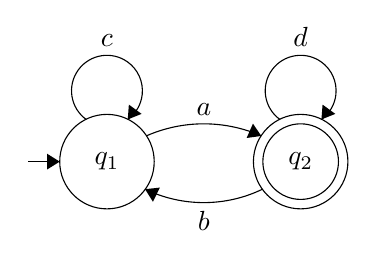
\begin{tikzpicture}[scale=0.2]
    \tikzstyle{every node}+=[inner sep=0pt]
    \draw [black] (5.2,-9.1) circle (3);
    \draw (5.2,-9.1) node {$q_1$};
    \draw [black] (17.5,-9.1) circle (3);
    \draw (17.5,-9.1) node {$q_2$};
    \draw [black] (17.5,-9.1) circle (2.4);
    \draw [black] (0.2,-9.1) -- (2.2,-9.1);
    \fill [black] (2.2,-9.1) -- (1.4,-8.6) -- (1.4,-9.6);
    \draw [black] (7.7,-7.466) arc (113.70628:66.29372:9.079);
    \fill [black] (15,-7.47) -- (14.47,-6.69) -- (14.07,-7.6);
    \draw (11.35,-6.2) node [above] {$a$};
    \draw [black] (15.081,-10.848) arc (-64.17666:-115.82334:8.565);
    \fill [black] (7.62,-10.85) -- (8.12,-11.65) -- (8.56,-10.75);
    \draw (11.35,-12.2) node [below] {$b$};
    \draw [black] (3.877,-6.42) arc (234:-54:2.25);
    \draw (5.2,-1.85) node [above] {$c$};
    \fill [black] (6.52,-6.42) -- (7.4,-6.07) -- (6.59,-5.48);
    \draw [black] (16.177,-6.42) arc (234:-54:2.25);
    \draw (17.5,-1.85) node [above] {$d$};
    \fill [black] (18.82,-6.42) -- (19.7,-6.07) -- (18.89,-5.48);
    \end{tikzpicture}
  \end{center}
  
  \textbf{Step 1:}
    
  Initial state $q_1$ has an incoming edge so create a new initial state $q_i$.
  \begin{center}
    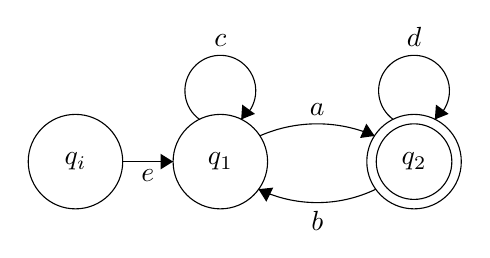
\begin{tikzpicture}[scale=0.2]
    \tikzstyle{every node}+=[inner sep=0pt]
    \draw [black] (12.4,-9.1) circle (3);
    \draw (12.4,-9.1) node {$q_1$};
    \draw [black] (24.7,-9.1) circle (3);
    \draw (24.7,-9.1) node {$q_2$};
    \draw [black] (24.7,-9.1) circle (2.4);
    \draw [black] (3.2,-9.1) circle (3);
    \draw (3.2,-9.1) node {$q_i$};
    \draw [black] (14.9,-7.466) arc (113.70628:66.29372:9.079);
    \fill [black] (22.2,-7.47) -- (21.67,-6.69) -- (21.27,-7.6);
    \draw (18.55,-6.2) node [above] {$a$};
    \draw [black] (22.281,-10.848) arc (-64.17666:-115.82334:8.565);
    \fill [black] (14.82,-10.85) -- (15.32,-11.65) -- (15.76,-10.75);
    \draw (18.55,-12.2) node [below] {$b$};
    \draw [black] (11.077,-6.42) arc (234:-54:2.25);
    \draw (12.4,-1.85) node [above] {$c$};
    \fill [black] (13.72,-6.42) -- (14.6,-6.07) -- (13.79,-5.48);
    \draw [black] (23.377,-6.42) arc (234:-54:2.25);
    \draw (24.7,-1.85) node [above] {$d$};
    \fill [black] (26.02,-6.42) -- (26.9,-6.07) -- (26.09,-5.48);
    \draw [black] (6.2,-9.1) -- (9.4,-9.1);
    \fill [black] (9.4,-9.1) -- (8.6,-8.6) -- (8.6,-9.6);
    \draw (7.8,-9.6) node [below] {$e$};
    \end{tikzpicture}
  \end{center}
  
  \textbf{Step 2:}
  
  Final state $q_2$ has an outgoing edge. So, create a new final state $q_f$.

  \begin{center}
    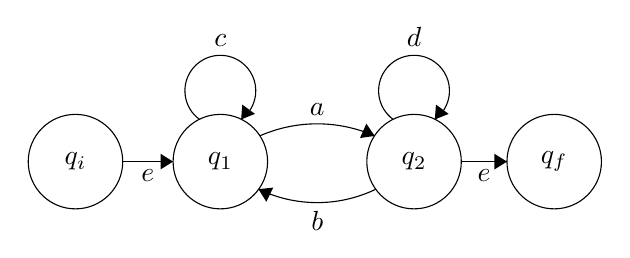
\begin{tikzpicture}[scale=0.2]
    \tikzstyle{every node}+=[inner sep=0pt]
    \draw [black] (12.4,-9.1) circle (3);
    \draw (12.4,-9.1) node {$q_1$};
    \draw [black] (24.7,-9.1) circle (3);
    \draw (24.7,-9.1) node {$q_2$};
    \draw [black] (3.2,-9.1) circle (3);
    \draw (3.2,-9.1) node {$q_i$};
    \draw [black] (33.6,-9.1) circle (3);
    \draw (33.6,-9.1) node {$q_f$};
    \draw [black] (14.9,-7.466) arc (113.70628:66.29372:9.079);
    \fill [black] (22.2,-7.47) -- (21.67,-6.69) -- (21.27,-7.6);
    \draw (18.55,-6.2) node [above] {$a$};
    \draw [black] (22.281,-10.848) arc (-64.17666:-115.82334:8.565);
    \fill [black] (14.82,-10.85) -- (15.32,-11.65) -- (15.76,-10.75);
    \draw (18.55,-12.2) node [below] {$b$};
    \draw [black] (11.077,-6.42) arc (234:-54:2.25);
    \draw (12.4,-1.85) node [above] {$c$};
    \fill [black] (13.72,-6.42) -- (14.6,-6.07) -- (13.79,-5.48);
    \draw [black] (23.377,-6.42) arc (234:-54:2.25);
    \draw (24.7,-1.85) node [above] {$d$};
    \fill [black] (26.02,-6.42) -- (26.9,-6.07) -- (26.09,-5.48);
    \draw [black] (6.2,-9.1) -- (9.4,-9.1);
    \fill [black] (9.4,-9.1) -- (8.6,-8.6) -- (8.6,-9.6);
    \draw (7.8,-9.6) node [below] {$e$};
    \draw [black] (27.7,-9.1) -- (30.6,-9.1);
    \fill [black] (30.6,-9.1) -- (29.8,-8.6) -- (29.8,-9.6);
    \draw (29.15,-9.6) node [below] {$e$};
    \end{tikzpicture}
  \end{center}

  \textbf{Step 3:}

  Start eliminating intermediate states

  \textbf{First eliminate $q_1$:}

  \quad There is a path going from $q_i$ to $q_2$ via $q_1$. So, after eliminating $q_1$ we can connect a direct path from $q_i$ to $q_2$ having cost: $e c^* a = c^* a$.

  \quad There is a loop on $q_2$ using state $q_i$. So, after eliminating $q_1$ we put a direct loop to $q_2$ having cost: $b c^* a$.

  After eliminating $q_1$, the FA looks like following
  \begin{center}
    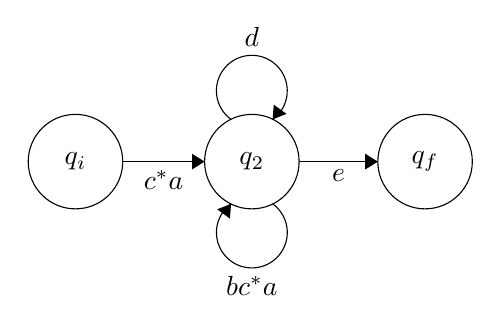
\begin{tikzpicture}[scale=0.2]
    \tikzstyle{every node}+=[inner sep=0pt]
    \draw [black] (14.4,-9.1) circle (3);
    \draw (14.4,-9.1) node {$q_2$};
    \draw [black] (3.2,-9.1) circle (3);
    \draw (3.2,-9.1) node {$q_i$};
    \draw [black] (25.4,-9.1) circle (3);
    \draw (25.4,-9.1) node {$q_f$};
    \draw [black] (13.077,-6.42) arc (234:-54:2.25);
    \draw (14.4,-1.85) node [above] {$d$};
    \fill [black] (15.72,-6.42) -- (16.6,-6.07) -- (15.79,-5.48);
    \draw [black] (17.4,-9.1) -- (22.4,-9.1);
    \fill [black] (22.4,-9.1) -- (21.6,-8.6) -- (21.6,-9.6);
    \draw (19.9,-9.6) node [below] {$e$};
    \draw [black] (6.2,-9.1) -- (11.4,-9.1);
    \fill [black] (11.4,-9.1) -- (10.6,-8.6) -- (10.6,-9.6);
    \draw (8.8,-9.6) node [below] {$c^*a$};
    \draw [black] (15.723,-11.78) arc (54:-234:2.25);
    \draw (14.4,-16.35) node [below] {$bc^*a$};
    \fill [black] (13.08,-11.78) -- (12.2,-12.13) -- (13.01,-12.72);
    \end{tikzpicture}
  \end{center}

  \textbf{Second eliminate $q_2$:}
  There is a direct path from $q_i$ to $q_f$ so, we can directly eliminate $q_2$ having cost.
  \begin{equation*}
    c^*a (d + bc^*a)^* e = c^*a (d + bc^*a)^*
  \end{equation*}
  which is our final regular expression for given finite automata.

\end{examplebreak}

\vfill\null
\columnbreak


\subsection{Languages that are and are not Regular}

To show that a language $L$ is regular, one of the following methods can be used:
\begin{itemize}
  \item write a regular expression $\alpha$ such that $L = L(\alpha)$
  \item construct an NFA $M$ such that $L = L(M)$
  \item use closure properties, e.g., for regular languages $L_1$ and $L_2$, show $L = L_1 \cap L_2$, $L = L_1 \cup L_2$, $L = L_1 L_2$,
  or $L = \Sigma^* \setminus L_1$ (more examples can be added)
\end{itemize}

There are two properties shared by all regular languages, but not by certain nonregular languages, may be phrased intuitively as follows: 
\begin{enumerate}
  \item As a string is scanned left to right, the amount of memory that is required in order to determine at the end whether or not the \textit{string is in the language must be bounded}, fixed in advance and dependent on the language, not the particular input string. For example, we would expect that $\{a^n b^n\ |\ n \geq 0\}$ is not regular, since it is difficult to imagine how a finite-state device could be constructed that would correctly remember, upon reaching the border between the $a$'s and the $b$'s, how many $a$'s it had seen, so that the number could be compared against the number of $b$'s.
  \item Regular languages with an infinite number of strings are represented by automata with cycles and regular expressions involving the Kleene star. Such languages must have infinite subsets with a certain simple repetitive structure that arises from the Kleene star in a corresponding regular expression or a cycle in the state diagram of a finite automaton. This would lead us to expect, for example, that $\{a^n\ |\ n \geq 1 \textnormal{ is a prime}\}$ is not regular, since there is no simple periodicity in the set of prime numbers.
\end{enumerate}

\noindent In brief,
\begin{formula}{}
  To show that a language $L$ is not regular, we use the following property of regular languages: 
  \begin{itemize}
    \item as a string is scanned from left to right, the amount of memory required to determine if $w \in L$ or $w \notin L$ must be bounded.
    \item In RL, infinite languages can be represented with Kleene star (cycle in automata), which induce a periodicity/pattern.
  \end{itemize}
\end{formula}

\end{multicols}

\newpage

\subsubsection{Pumping Lemma}

These intuitive ideas are formalized in the following theorem known as \textit{Pumping Lemma}.

\begin{theorem}{: Pumping Lemma}
  Let $L$ be a regular language. There is an integer $n \geq 1$ such that any string $w \in L$ with $|w| \geq n$ can be rewritten as $w = xyz$ such that $y \neq e$, $|xy| \leq n$ and $xy^iz \in L$ for each $i \geq 0$. 
\end{theorem}

\begin{formula}{}
  \quad Assume $L$ is a regular language and there is a string $w \in L$. Now, imagine, not find or determine, that there is a integer $n$ that is $n \geq 1$, $n > 0$. Also, this integer is smaller than the length of the string $w$, $n \leq |w|$. So,
\begin{align*}
  |w| \geq n \geq 1 && \textnormal{or} && |w| \geq n > 0
\end{align*}
Also, notice that the string can be written as three parts: $w = xyz$.

If the followings are satisfied, it shows that $w \in L$ and $L$ is regular:
\begin{itemize}
  \item $|y| > 0$: $y$ is not empty string
  \item $|xy| \leq n$: the length of the part of the string $xy$ is less than $n$
  \item $xy^iz \in L,\textnormal{ for each } i \geq 0$: When part $y$ is repeated, or pumped, as many times we want, the expression is still in language
\end{itemize}
In here, $x$ or $z$ can be empty string, $e$, but $y$ cannot be the empty string, $e$. Notice that the chosen part of string that will be compared with $n$ should be located in first $n$.
\end{formula}

Pumping lemma is also used to show that a language is not regular: start applying the pumping lemma, then find a contradiction.
\begin{formula}{}
\noindent For each regular language $L$,

\quad there exists $n \geq 1$ such that (this is a general term do not pick a number!!!)

\quad \quad for each $w \in L$ with $|w| \geq n$ (write/pick a string with respect to $n$, that can be used to reach a contradiction)

\quad \quad \quad there exists $x, y, z$ with $w = xyz$, $y \neq e$, $|xy| \leq n$ (consider each possible split satisfying these constraints)

\quad \quad \quad \quad for each $i \geq 0$, $xy^iz \in L$ (show that there exists an $i$ such that $xy^iz \neq L$, contradiction)
\end{formula}


\subsection{State Minimization}

The process of reducing a given DFA to its minimal form is called as minimization of DFA.
\begin{itemize}
  \item It contains the minimum number of states.
  \item The DFA in its minimal form is called as a Minimal DFA.
\end{itemize}

\noindent The two popular methods for minimizing a DFA are
\begin{itemize}
  \item Equivalence Theorem
  \item Myhill Nerode Theorem
\end{itemize}

\noindent Since Myhill Nerode Theorem is a little bit cumbersome and prone to error compared to Equivalence Theorem, it is better to focus on the Equivalence Theorem.

\newpage
\subsubsection{Equivalence Theorem}

\begin{multicols}{2}
\setlength{\columnsep}{1.5cm}
\setlength{\columnseprule}{0.2pt}

The steps as follows:
\begin{enumerate}
  % Step 1
  \item Eliminate all the dead states and inaccessible states from the given DFA (if any).
    \begin{itemize}
      \item \textbf{Dead State:} All those non-final states which transit to itself for all input symbols in $\Sigma$ are called as dead states.
      \item \textbf{Inaccessible State:} All those states which can never be reached from the initial state are called as inaccessible states.
    \end{itemize}
  
  % Step 2
  \item Draw a state transition table for the given DFA. Transition table shows the transition of all states on all input symbols in $\Sigma$.
  
  % Step 3
  \item Now, start applying equivalence theorem.
    \begin{itemize}
      \item Take a counter variable $k$ and initialize it with value 0.
      \item Divide $Q$ (\textit{set of states}) into two sets such that one set contains all the non-final states and other set contains all the final states.
      \item This partition is called $P_0$.
    \end{itemize}
  
  % Step 4
  \item 
    \begin{itemize}
      \item Increment $k$ by $1$.
      \item Find $P_k$ by partitioning the different sets of $P_{k - 1}$.
      \item In each set of $P_{k - 1}$, consider all the possible pair of states within each set and if the two states are distinguishable, partition the set into different sets in $P_k$.
    \end{itemize}
  
    Two states $q_1$ and $q_2$ are distinguishable in partition $P_k$ for any input symbol `$a$', if $\delta(q_1, a)$ and $\delta(q_2, a)$ are in different sets in partition $P_{k-1}$.
  
  % Step 5
  \item Repeat \textit{step-4} until no change in partition occurs. In other words, when you find $P_k = P_{k - 1}$, stop.
  
  % Step 6
  \item All those states which belong to the same set are equivalent. The equivalent states are merged to form a single state in the minimal DFA.
    \begin{center}
      \textit{\# of states in Minimal DFA = \# of sets in $P_k$  }
    \end{center}
\end{enumerate}

\end{multicols}
